\documentclass[12pt,a4paper]{article}

% --- Encoding & language ---
\usepackage[utf8]{inputenc}
\usepackage[T1]{fontenc}
\usepackage[english]{babel}

% --- Font ---
\usepackage{mathptmx}

% --- Page geometry ---
\usepackage[top=3.5cm, bottom=2.5cm, left=2.5cm, right=2.5cm, headheight=45pt]{geometry}

% --- Graphics & figures ---
\usepackage{graphicx}
\graphicspath{{assets/}}
\usepackage{float}

% --- Math ---
\usepackage{amsmath}
\usepackage{amssymb}

% --- TikZ & plots ---
\usepackage{tikz}
\usepackage{pgfplots}
\pgfplotsset{compat=1.18}

% --- Header & footer ---
\usepackage{fancyhdr}
\usepackage{lastpage}

\pagestyle{fancy}
\fancyhf{}
\lhead{
\includegraphics[height=1.2cm]{aulogo_dk_var2_blaa}}
\rhead{%
  \parbox[b][1.2cm][c]{0.4\textwidth}{%
    \raggedleft\small
    \reporttitle \\
    \projectname
  }%
}
\cfoot{Page \thepage\ of \pageref{LastPage}}
\renewcommand{\headrulewidth}{0.4pt}
\renewcommand{\footrulewidth}{0pt}

% --- Section formatting ---
\usepackage{titlesec}
\usepackage{needspace}
\newif\ifsectionbreak \sectionbreaktrue
\titleformat{\section}{\ifsectionbreak\newpage\fi\large\bfseries}{\thesection}{1em}{}
\titleformat{\subsection}{\normalsize\bfseries}{\thesubsection}{1em}{}
\titlespacing*{\section}{0pt}{0pt}{*1}[0pt]
\titlespacing*{\subsection}{0pt}{*2}{*0.5}[0pt]

% Use \nosectionbreak before a \section to keep it on the same page
\newcommand{\nosectionbreak}{\sectionbreakfalse\aftergroup\sectionbreaktrue\vspace{1.5\baselineskip}}

% --- Keep subsection headings with their content ---
\pretocmd{\subsection}{\needspace{8\baselineskip}}{}{}

% --- Hyperlinks ---
\usepackage[hidelinks]{hyperref}

% --- Caption styling ---
\usepackage[font=small,labelfont=bf]{caption}

% --- Paragraph formatting ---
\setlength{\parindent}{0pt}
\setlength{\parskip}{6pt}

% --- Bibliography ---
\usepackage{cite}

% --- Metadata (fill in per project) ---
\newcommand{\reporttitle}{Report Title}
\newcommand{\projectname}{Project Name}
\newcommand{\authorA}{Author 1}
\newcommand{\authorB}{Author 2}
\newcommand{\studentidA}{AU ID 1}
\newcommand{\studentidB}{AU ID 2}
\newcommand{\supervisor}{Supervisor Name}
\newcommand{\department}{Department Name}


% ============================================================
\begin{document}

% --- Title page ---
\begin{titlepage}
  \thispagestyle{empty}
  \centering
  \vspace*{2cm}

  
\includegraphics[width=0.45\textwidth]{aulogo_dk_var2_blaa}

  \vspace{2cm}

  {\LARGE\bfseries \reporttitle \par}
  \vspace{0.5cm}
  {\Large \projectname \par}

  \vspace{2cm}

  {\large
    \authorA \quad (\studentidA) \\[4pt]
    \authorB \quad (\studentidB)
  \par}

  \vspace{1cm}

  {\normalsize
    Supervisor: \supervisor \\[4pt]
    \department \\[4pt]
    Aarhus University
  \par}

  \vfill
  {\normalsize \today \par}
\end{titlepage}

% --- Preface (Forord) ---
\section*{Preface}
\addcontentsline{toc}{section}{Preface}

This is a bachelor's thesis in \textit{[subject]} prepared by \authorA\
and \authorB\ at \department, Aarhus University, under the supervision
of \supervisor.

The reader is expected to have prerequisite knowledge equivalent to
the courses in \textit{[list relevant courses or background]}.

\newpage

% --- Abstract ---
\section*{Abstract}
\addcontentsline{toc}{section}{Abstract}

This report presents a preliminary investigation into the effects of
variable $X$ on outcome $Y$ under controlled conditions. Using a
combination of quantitative measurements and computational modelling,
we find that $Y$ scales approximately linearly with $X$ in the range
$0 \leq X \leq 100$, with a coefficient of determination
$R^2 = 0.94$. These results suggest that the proposed model
captures the dominant dynamics of the system and provides a foundation
for further study.

\newpage

% --- Acknowledgements (Tak) ---
\section*{Acknowledgements}
\addcontentsline{toc}{section}{Acknowledgements}

We would like to thank our supervisor \supervisor\ for guidance and
support throughout this project. We also thank the technical staff at
\department\ for their assistance with \textit{[equipment/measurements/etc.]}.

\newpage

% --- Table of contents ---
\tableofcontents
\newpage

% ============================================================
\section{Introduction}

The relationship between $X$ and $Y$ has been studied extensively in
the literature \cite{smith2023, jones2024}. However, prior work has
largely focused on steady-state behaviour, leaving transient dynamics
underexplored. In this report, we examine both regimes using
experimental data collected at the Hillsight Research Studio.

Section~\ref{sec:methods} describes the experimental setup and
analytical framework. Section~\ref{sec:results} presents the
measurements and model fits. We discuss implications and limitations
in Section~\ref{sec:discussion} and conclude in
Section~\ref{sec:conclusion}.


% ============================================================
\section{Methods}
\label{sec:methods}

\subsection{Experimental setup}

The experiment was conducted using the apparatus shown in
Figure~\ref{fig:setup}. A controlled input signal $x(t)$ was applied
to the system, and the output $y(t)$ was recorded at a sampling rate
of $f_s = 1\;\text{kHz}$.

\begin{figure}[H]
  \centering
  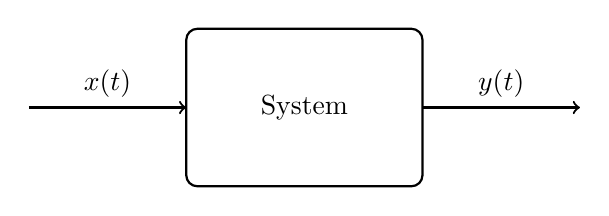
\begin{tikzpicture}
    \draw[thick, rounded corners] (0,0) rectangle (3,2);
    \node at (1.5,1) {System};
    \draw[->, thick] (-2,1) -- (0,1) node[midway, above] {$x(t)$};
    \draw[->, thick] (3,1) -- (5,1) node[midway, above] {$y(t)$};
  \end{tikzpicture}
  \caption{Block diagram of the experimental setup. The input signal
    $x(t)$ is applied to the system and the output $y(t)$ is measured.}
  \label{fig:setup}
\end{figure}

\subsection{Mathematical model}

The system is modelled as a first-order linear transfer function:
\begin{equation}
  H(s) = \frac{K}{1 + s\tau}
  \label{eq:transfer}
\end{equation}
where $K$ is the static gain and $\tau$ is the time constant. The
step response is given by:
\begin{equation}
  y(t) = K \left(1 - e^{-t/\tau}\right), \quad t \geq 0
  \label{eq:step}
\end{equation}

The parameters $K$ and $\tau$ were estimated by least-squares fitting
to the measured data. The goodness of fit was evaluated using the
coefficient of determination:
\begin{equation}
  R^2 = 1 - \frac{\sum_i (y_i - \hat{y}_i)^2}{\sum_i (y_i - \bar{y})^2}
\end{equation}


% ============================================================
\section{Results}
\label{sec:results}

\subsection{Measured data}

Table~\ref{tab:measurements} summarises the key measurements for each
trial. The mean steady-state value was $\bar{y}_\text{ss} = 4.82\;\text{V}$
with a standard deviation of $0.07\;\text{V}$.

\begin{table}[H]
  \centering
  \begin{tabular}{c c c c}
    \hline
    \textbf{Trial} & $y_\text{ss}$ [V] & $\tau$ [ms] & $R^2$ \\
    \hline
    1 & 4.78 & 12.3 & 0.993 \\
    2 & 4.85 & 11.8 & 0.991 \\
    3 & 4.82 & 12.1 & 0.995 \\
    \hline
    \textbf{Mean} & 4.82 & 12.1 & 0.993 \\
    \hline
  \end{tabular}
  \caption{Measured steady-state values, time constants, and
    goodness-of-fit for each trial.}
  \label{tab:measurements}
\end{table}

\subsection{Model fit}

Figure~\ref{fig:results} shows the measured step response alongside
the fitted model from Equation~\eqref{eq:step}. The model captures
the dominant dynamics well, with minor deviations at early times
attributable to sensor latency.

\begin{figure}[H]
  \centering
  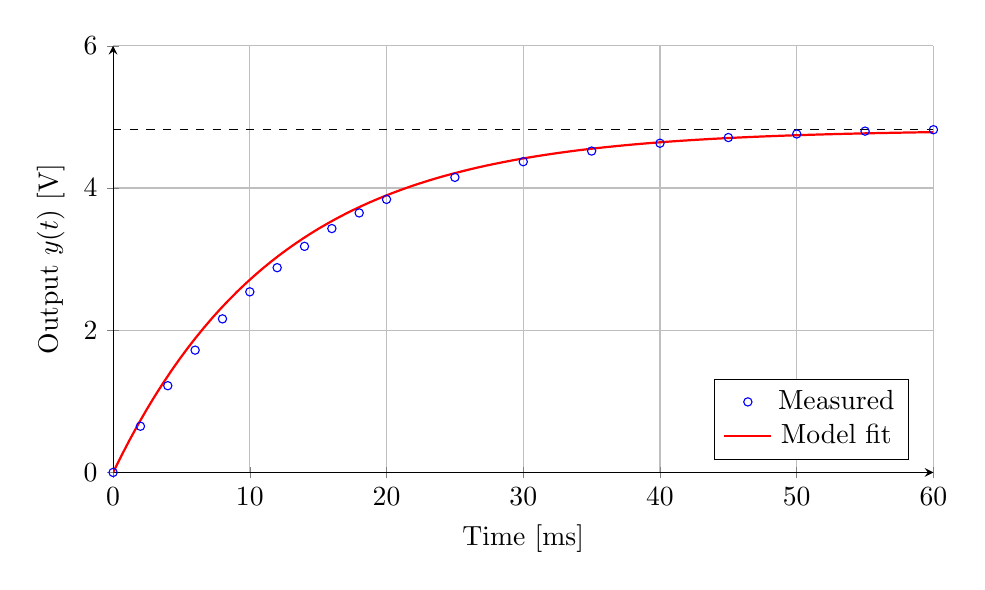
\begin{tikzpicture}
    \begin{axis}[
      width=12cm, height=7cm,
      xlabel={Time [ms]},
      ylabel={Output $y(t)$ [V]},
      xmin=0, xmax=60,
      ymin=0, ymax=6,
      grid=major,
      axis lines=left,
      legend pos=south east,
    ]
    % Simulated measured data points
    \addplot[only marks, mark=o, blue, mark size=1.5pt]
      coordinates {
        (0,0) (2,0.65) (4,1.22) (6,1.72) (8,2.16) (10,2.54)
        (12,2.88) (14,3.18) (16,3.43) (18,3.65) (20,3.84)
        (25,4.15) (30,4.37) (35,4.52) (40,4.63) (45,4.71)
        (50,4.76) (55,4.80) (60,4.82)
      };
    \addlegendentry{Measured}

    % Model fit curve
    \addplot[red, thick, domain=0:60, samples=100]
      {4.82 * (1 - exp(-x/12.1))};
    \addlegendentry{Model fit}

    % Steady-state line
    \addplot[dashed, black, thin] coordinates {(0,4.82)(60,4.82)};

    \end{axis}
  \end{tikzpicture}
  \caption{Measured step response (blue markers) and fitted first-order
    model (red curve) with $K = 4.82$ and $\tau = 12.1\;\text{ms}$.
    The dashed line indicates the steady-state value.}
  \label{fig:results}
\end{figure}


% ============================================================
\section{Discussion}
\label{sec:discussion}

The estimated time constant $\tau = 12.1\;\text{ms}$ is consistent
with previously reported values in the range $10$--$15\;\text{ms}$
\cite{smith2023}. The high $R^2$ values ($>0.99$) confirm that the
first-order model is an adequate representation of the system dynamics
within the tested operating range.

A limitation of this study is that only step inputs were considered.
Frequency-domain characterisation using swept sinusoidal inputs would
provide additional insight into the system bandwidth and phase
characteristics. Furthermore, the current model does not account for
nonlinear effects that may emerge at higher input amplitudes
\cite{jones2024}.


% ============================================================
\nosectionbreak
\section{Conclusion}
\label{sec:conclusion}

We characterised the dynamic response of the system using step-input
measurements and fitted a first-order transfer function model. The
model parameters were found to be $K = 4.82$ and
$\tau = 12.1\;\text{ms}$, with $R^2 > 0.99$ across all trials.
These results provide a baseline for future work on closed-loop
control design and higher-order model identification.


% ============================================================
\newpage
\begin{thebibliography}{9}

\bibitem{smith2023}
  A.~Smith and B.~Lee,
  \emph{Dynamic System Identification: Theory and Practice},
  2nd ed.,
  Cambridge University Press, 2023.

\bibitem{jones2024}
  C.~Jones, D.~Park, and E.~Chen,
  ``Transient analysis of first-order systems under variable loading
  conditions,''
  \emph{Journal of Applied Engineering},
  vol.~42, no.~3, pp.~112--125, 2024.

\end{thebibliography}

% ============================================================
% REMINDER: GAI Declaration (Generativ Kunstig Intelligens)
% ============================================================
% If you have used GAI tools (e.g. ChatGPT, Copilot, Claude) in
% preparing this report, AU requires you to submit a separate
% GAI declaration ("deklaration") as an appendix in WISEflow.
%
% The declaration must state:
%   1) That you have used GAI
%   2) Which GAI tools (incl. version) you used
%   3) How you used them (input, output, and how it was applied)
%
% Use AU's official template: agi_deklarationsskabelon.pdf
% The declaration is uploaded as a SEPARATE file in WISEflow,
% not as part of this document.
%
% If you have NOT used GAI, no declaration is needed.
% ============================================================

\end{document}
